%! Author = inma, germán, isaac, natan
%! Date = 2025-07-11

\documentclass[12pt]{beamer}
\usetheme{Madrid}
\usecolortheme{default}

\usepackage{amsmath}
\usepackage{amsthm}
\usepackage{amsfonts}
\usepackage[utf8]{inputenc}
\usepackage[spanish, english]{babel}
\usepackage{color}
\usepackage{float}
\usepackage{tikz}

\setbeamertemplate{frametitle}{
  \vspace*{0.5em}
  \insertframetitle
  \vspace*{0.5em}
}
\setbeamercolor{frametitle}{fg=black}
\setbeamertemplate{background}{
\ifnum\insertpagenumber=1
    \begin{tikzpicture}[remember picture,overlay]
    \node[anchor=north west, xshift=-1cm, yshift=1.3cm, opacity=0.2]
        at (current page.north west) {
        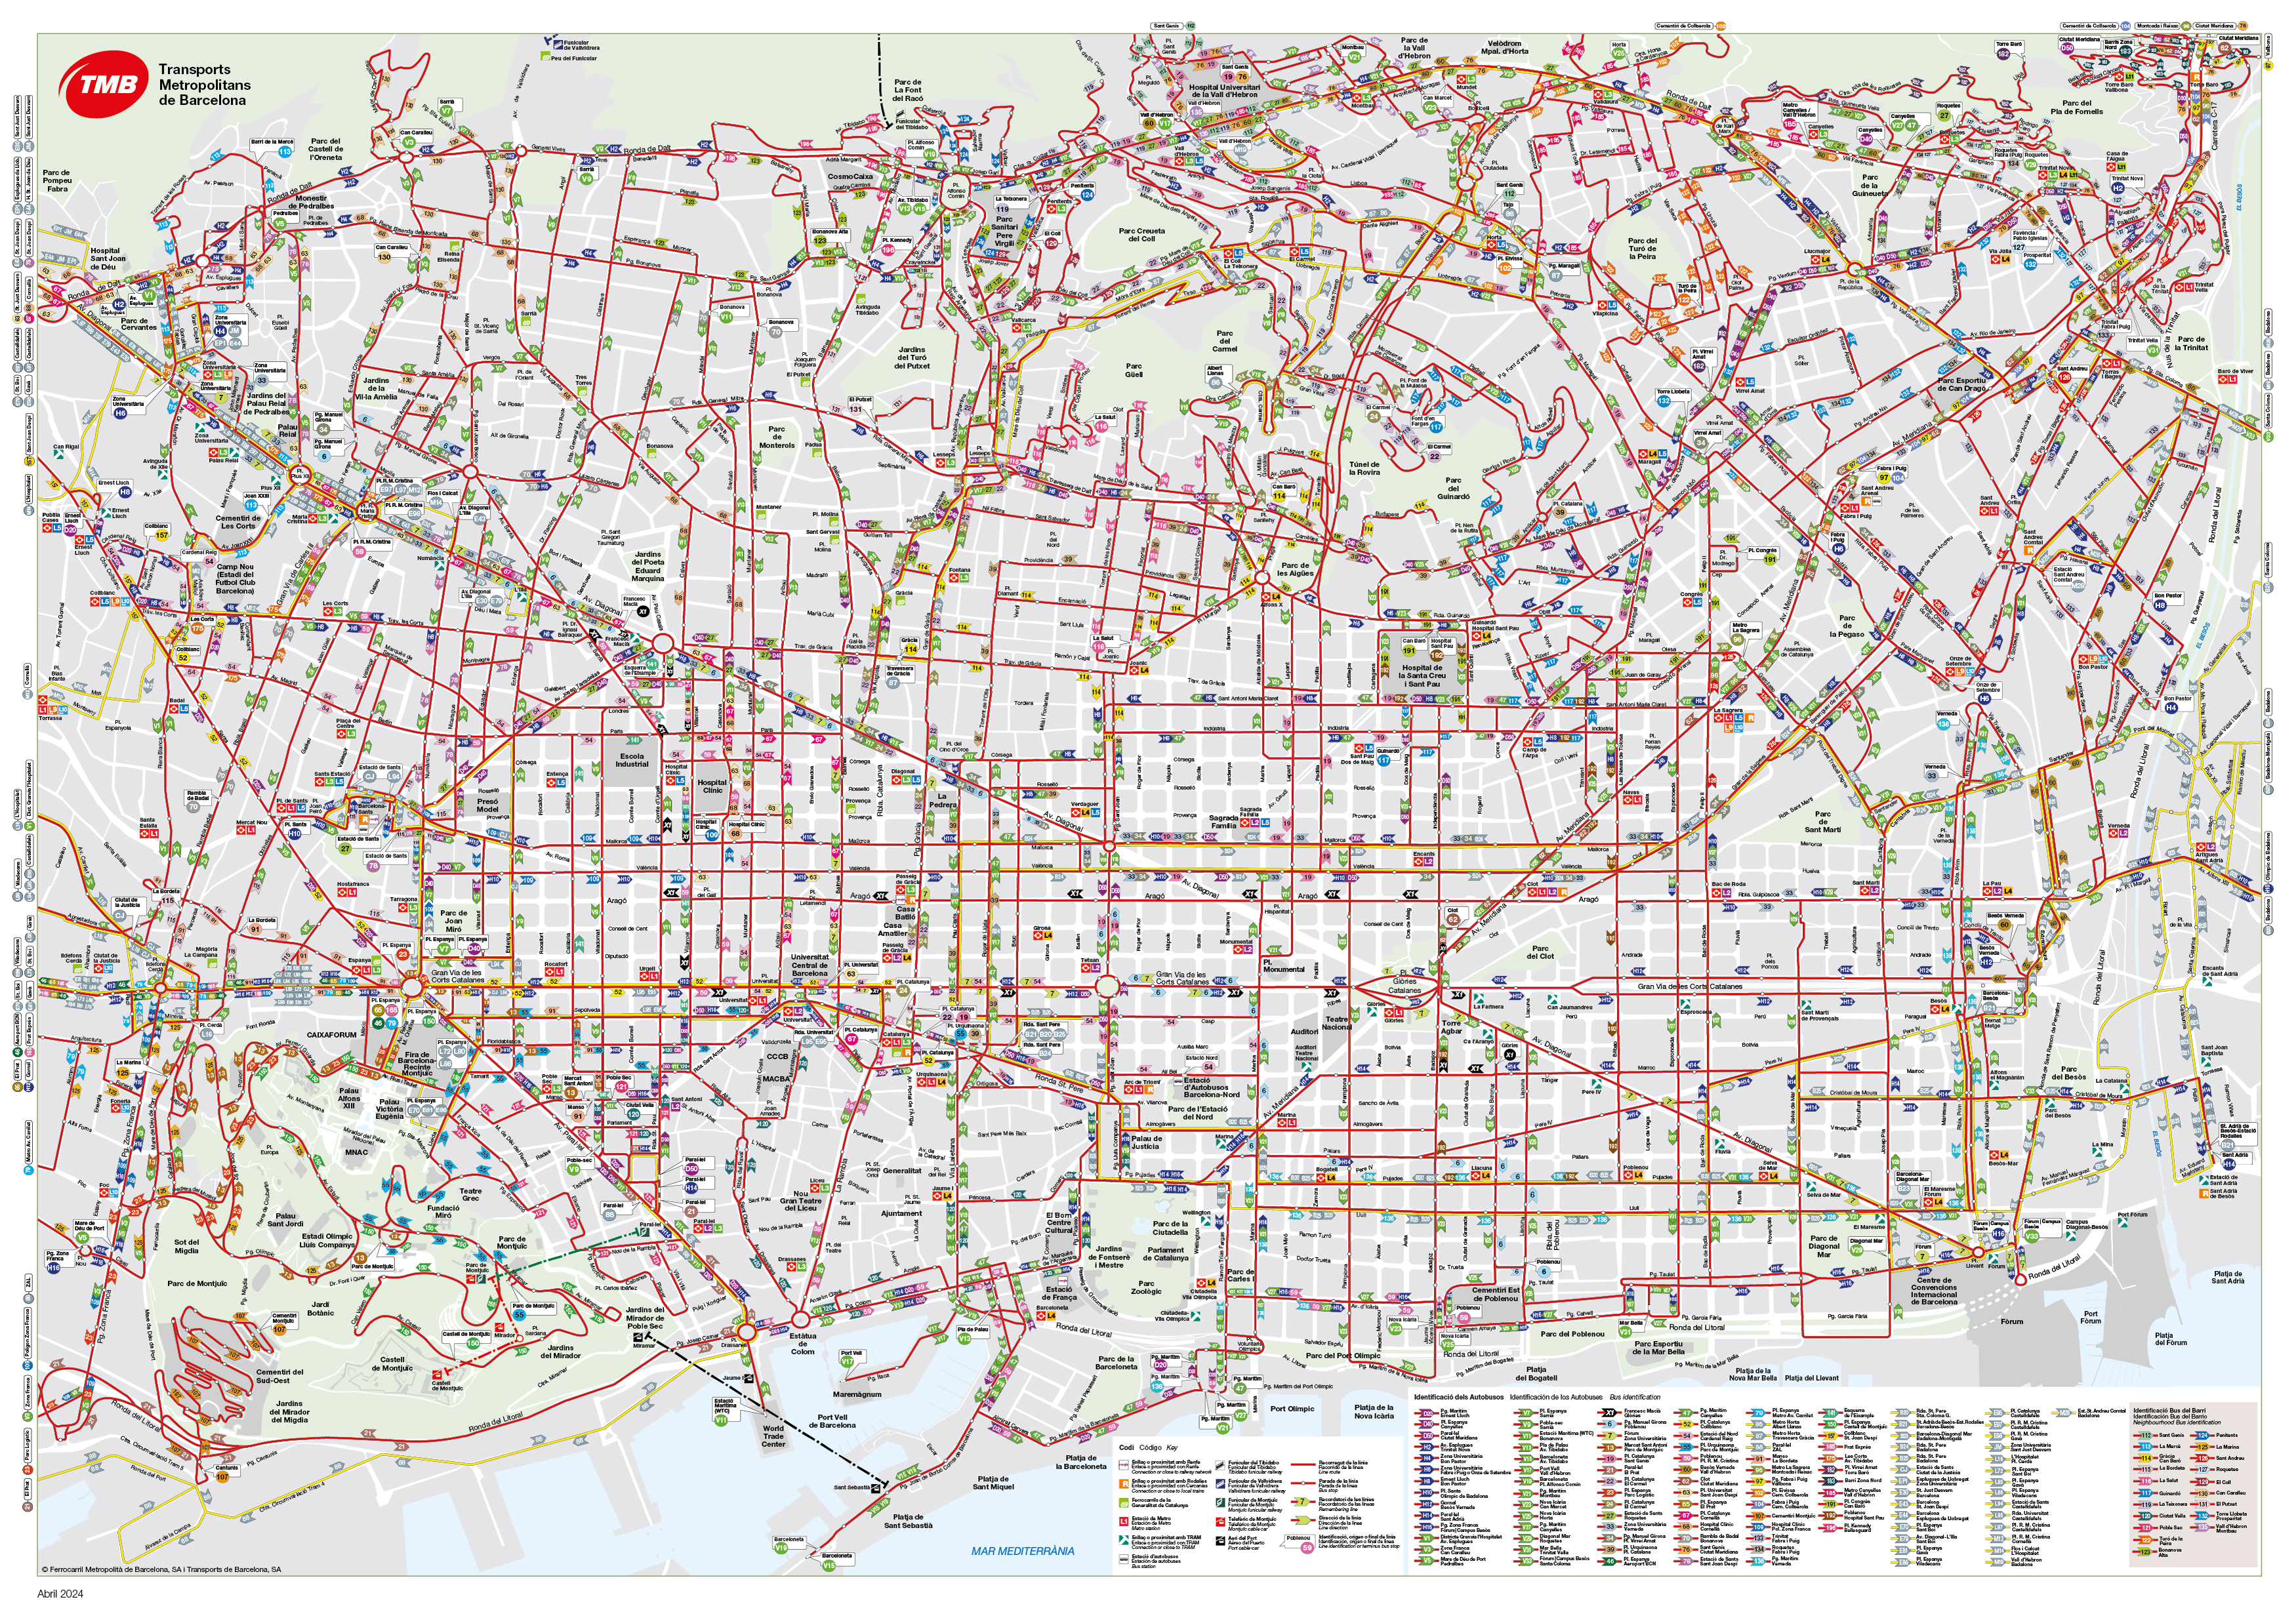
\includegraphics[width=1.5\paperwidth]{images/bcn_map}
    };
    \end{tikzpicture}
\else
    \begin{tikzpicture}[remember picture,overlay]
    \node[anchor=north west, xshift=-0.2cm, yshift=0.2cm, opacity=0.4]
        at (current page.north west) {
        \includegraphics[width=\paperwidth]{images/map_bg}
    };
    \end{tikzpicture}
\fi
}

\setbeamertemplate{footline}
{
  \leavevmode%
  \hbox{%
  \begin{beamercolorbox}[wd=.333333\paperwidth,ht=2.25ex,dp=1ex,center]{author in head/foot}%
    \usebeamerfont{author in head/foot}\insertinstitute
  \end{beamercolorbox}%
  \begin{beamercolorbox}[wd=.333333\paperwidth,ht=2.25ex,dp=1ex,center]{title in head/foot}%
    \usebeamerfont{title in head/foot}\inserttitle
  \end{beamercolorbox}%
  \begin{beamercolorbox}[wd=.333333\paperwidth,ht=2.25ex,dp=1ex,right]{date in head/foot}%
    \usebeamerfont{date in head/foot}\insertshortdate{}\hspace*{2em}
    \insertframenumber{} / \inserttotalframenumber\hspace*{2ex}
  \end{beamercolorbox}}%
  \vskip0pt%
}

\title{Efficient Bus Allocation}
\subtitle{XI Iberian Modeling Week}
\author{Inmaculada Fernández \and Germán López \and Isaac Martínez \and Natan Sisoev}
\date{11th July 2025}
\institute{Centre de Recerca Matemàtica}

\begin{document}

\frame{\titlepage}

\begin{frame}
\frametitle{Index}
\tableofcontents
\end{frame}

\begin{frame}
\begin{center}
\Huge{Problem Statement}
\end{center}
\end{frame}

\section{Problem Statement}
\begin{frame}
\frametitle{Problem Statement}
For public transport companies, it is important to determine the hourly number of buses required to meet passenger demand throughout a typical day.

\vspace{0.3cm}
Given a forecast of daily demand patterns and origin-destination data, the challenge involves estimating trip durations by modeling factors such as:
\begin{itemize}
\item Bus movement
\item Route alignment
\item Boarding times
\item Stop frequency
\end{itemize}

\vspace{0.3cm}
To ensure efficient and eco-conscious operations, participants must also consider synchronization strategies between buses to reduce waiting and travel times, aiming to minimize fleet size, fuel consumption, and environmental impact.
\end{frame}

\begin{frame}
\begin{center}
\Huge{Model Considerations}
\end{center}
\end{frame}

\section{Model Considerations}
\begin{frame}
\frametitle{Model Considerations - Building Complexity}
We develop our model by progressively adding real-world complexity:

\vspace{0.5cm}
\begin{enumerate}
\item \textbf{Free Movement} - Theoretical baseline with constant speed
\item \textbf{Bus Stops} - Adding acceleration/deceleration dynamics
\item \textbf{Dwell Time} - Passenger boarding and alighting
\item \textbf{Traffic Lights} - Urban infrastructure delays
\item \textbf{Traffic} - Vehicle interactions and congestion
\end{enumerate}

\vspace{0.5cm}
\textbf{Approach}: From theoretical foundations to practical implementation, transitioning from stochastic modeling to deterministic simulation using expected values.
\end{frame}

\subsection{Free Movement}
\begin{frame}
\frametitle{Free Movement - Baseline}
\textbf{Simplest Case}: Constant velocity along the entire route

\vspace{0.3cm}
\textbf{Route Characteristics}:
\begin{itemize}
\item Total distance: 11.5 km
\item Maximum legal speed: 50 km/h
\item Almost straight road (no turning delays)
\end{itemize}

\vspace{0.3cm}
\textbf{Travel Time Calculation}:
\begin{equation}
T_{\text{free}} = \frac{D}{v_{\text{max}}} = \frac{11.5 \text{ km}}{50 \text{ km/h}} = 0.23 \text{ h} = 13.8 \text{ min}
\end{equation}

\vspace{0.3cm}
This provides our theoretical minimum travel time, serving as a baseline for measuring the impact of real-world factors.
\end{frame}

\subsection{Bus Stops}
\begin{frame}
\frametitle{Bus Stops - Braking and Speeding Up}
\textbf{Physical Constraints}:
\begin{itemize}
\item 34 bus stops along the route
\item Smooth acceleration and deceleration profiles
\item Constant braking/acceleration distances
\end{itemize}

\vspace{0.3cm}
\textbf{Key Parameters}:
\begin{align}
t_a &= \text{Acceleration time}  \notag\\
t_d &= \text{Deceleration time}  \notag\\
d_p &= \text{Distance lost per stop (braking + acceleration)}  \notag\\
n_p &= \text{Number of stops} = 34 \notag
\end{align}

\vspace{0.3cm}
\textbf{Modified Travel Time}:
\begin{equation}
T_{\text{stops}} = \frac{D - (n_p-1)d_p}{v_m} + (n_p-1)(t_a + t_d)
\end{equation}
\end{frame}

\subsection{Dwell Time}
\begin{frame}
\frametitle{Dwell Time - Passenger Interactions}
\textbf{Definition}: Time spent at each stop for passenger boarding/alighting

\vspace{0.3cm}
\textbf{Stochastic Model}:
\begin{align}
t_0 &= \text{Base door opening and closing time}  \notag\\
\alpha &= \text{Time per passenger (boarding/alighting)}  \notag\\
N_{ip} &\sim \mathcal{N}(\mu_{ip}, \sigma_{ip}^2)  \notag\\
N_{ip} &= \text{Number of passengers at stop } i \notag \\
W_i &= t_0 + N_{ip} \cdot \alpha  \notag
\end{align}

\vspace{0.3cm}
\textbf{Total Travel Time}:
\begin{equation}
T_{\text{total}} = \frac{D - (n_p-1)d_p}{v_m} + (n_p-1)(t_a + t_d) + \sum_{i=1}^{n_p} W_i
\end{equation}
\end{frame}

\subsection{Traffic Lights}
\begin{frame}
\frametitle{Traffic Lights - Urban Infrastructure}
\textbf{Synchronization Model}:
\begin{itemize}
\item Traffic lights are synchronized when encountered consecutively
\item Synchronization breaks at bus stops
\item Each inter-stop segment has probability $\frac{1}{2}$ of encountering a red light
\end{itemize}

\vspace{0.3cm}
\textbf{Random Variables}:
\begin{align}
S_i &\sim \text{Bernoulli}(p = 0.5) \quad \text{(encounter red light)}  \notag\\
t_{tl} &\sim \mathcal{U}(0, 60) \quad \text{(waiting time at red light)}  \notag\\
n_{tl} &\sim \text{Binomial}(33, 0.5) \quad \text{(total red lights encountered)} \notag
\end{align}

\vspace{0.3cm}
\textbf{Extended Model}:
\begin{equation}
T_{\text{lightstotal}} = T_{\text{total}} + \sum_{i=1}^{n_p} S_i \cdot t_{tl,i}
\end{equation}
\end{frame}

\subsection{Traffic}
\begin{frame}
\frametitle{Traffic - Vehicle Interactions}
\textbf{Congestion Effects}:
\begin{itemize}
\item Reduced average speed during peak hours
\item Probability of encountering slower vehicles
\item Speed depends on passenger density and time of day
\end{itemize}

\vspace{0.3cm}
\textbf{Stochastic Speed Model}:
\begin{align}
C_i &\sim \text{Bernoulli}\left(\frac{\sum_j N_{p_j}(h)}{\max_{\hat{h}}(\sum_j N_{p_j}(\hat{h}))} \cdot \frac{N_{p_i}}{\max_j(N_{p_j}(h))}\right)  \notag\\
\hat{v}_i &\sim \mathcal{N}(\mu(h), \sigma^2)  \notag\\
v_i &= C_i \cdot \hat{v}_i + (1-C_i) \cdot v_M  \notag\\
\mu(h) &= v_M - \gamma N_p(h) \notag
\end{align}

Where $C_i$ represents encountering congestion, $\hat{v}_i$ is the reduced speed, and $\mu(h)$ is the hour-dependent expected speed.
\end{frame}


\begin{frame}
\frametitle{Traffic - Vehicle Interactions}


\textbf{Integrating factors:}

\begin{itemize}
    \item Distance covered when accelerating
    \item Traffic stop time as a limit in velocity
    \item Factors occur independently in-between stops
\end{itemize}
\vspace{0.5cm}
\textbf{Stochastic complete model:}
\begin{equation}
    T_t=(n_p-1)(t_a+t_d)+\sum_{i=1}^{n_p} [W_i + d_i/v_i +S_i\cdot (t_{s_i}+\max({t_a+t_d-d_{p}/v_i},0))]
\end{equation}

\end{frame}


\begin{frame}
\begin{center}
\Huge{From Stochastic to Deterministic}
\end{center}
\end{frame}

\section{From Stochastic to Deterministic}
\begin{frame}
\frametitle{Transition to Deterministic Model}
\textbf{Motivation}: Simplify complex stochastic simulation using expected values

\vspace{0.3cm}
\textbf{Key Simplifications}:
\begin{itemize}
\item \textbf{Traffic Lights Duration}: $E[t_{tl}] = 30$ seconds (uniform distribution)
\item \textbf{Red Lights Encounters}: $E[n_{tl}] = 32 \times 0.5 = 16$ lights
\item \textbf{Traffic Speed}: $E[v_i] = P(\text{traffic}) \cdot E[\hat{v}_i] + P(\text{no traffic}) \cdot v_M$
\end{itemize}

\vspace{0.3cm}
\textbf{Expected Travel Time}:
\begin{multline}
E[T_{\text{total}}] = (n_p-1)(t_a + t_d) + n_p t_0 + \alpha \sum_{i=1}^{n_p} E[n_{ip}] \\
+ \sum_{i=1}^{n_p} \frac{d_i}{E[v_i]} + E[n_{tl}] \cdot E[t_{tl}]
\end{multline}
\end{frame}

\begin{frame}
\frametitle{Practical Implementation}
\textbf{Deterministic Simulation}: Using expected values eliminates randomness while maintaining model accuracy

\vspace{0.3cm}
\textbf{Implementation Benefits}:
\begin{itemize}
\item Reproducible results
\item Faster computation
\item Easier parameter sensitivity analysis
\end{itemize}

\vspace{0.3cm}
\textbf{Model Parameters}:
\begin{align}
t_0 &= 5 \text{ seconds (door opening)} \notag\\
\alpha &= 2 \text{ seconds per passenger} \notag\\
t_a = 2 t_d &= 10 \text{ seconds (acceleration/deceleration time)} \notag\\
E[t_{tl}] &= 30 \text{ seconds (traffic light delay)} \notag\\
\gamma &= 1 / 120 \text{ m$\cdot$s$^{-1}\cdot$passenger$^{-1}$ (passengers coefficient)} \notag
\end{align}
\end{frame}

\begin{frame}
\frametitle{Smooth Acceleration Model}

\textbf{Goal:} Interpolate a smooth velocity profile during acceleration.

\vspace{0.3cm}
\textbf{Conditions:}
\begin{itemize}
  \item Initial position: $x = 0$, with $v = 0$, $a = 0$
  \item Final time: $t = t_a$ with $x = x_f$, $v = v_{\text{max}}$, $a = 0$
  \item Use a degree-3 polynomial for velocity: $$v(t) = a_3 t^3 + a_2 t^2 + a_1 t + a_0$$
\end{itemize}

\vspace{0.3cm}
\textbf{Why cubic?}
\begin{itemize}
  \item Enough degrees of freedom to match position, velocity, and acceleration constraints
  \item Ensures continuous acceleration → smoother gas supply and realistic dynamics
\end{itemize}
\end{frame}

\begin{frame}
\begin{center}
\Huge{Results}
\end{center}
\end{frame}

\section{Results}

\begin{frame}
\frametitle{Dwell Time Analysis}
Using the dwell time formula $W_i = t_0 + n_{ip}\alpha$:

\vspace{0.5cm}
\textbf{Peak Hour (17:00 - 980 passengers):}
\begin{align}
\text{Total dwell time} &= 34 \times 4 + 980 \times 2 \notag\\
&= 136 + 1960 \notag\\
&= 2096 \text{ seconds} \notag\\
&= 34.93 \text{ minutes} \notag
\end{align}

\vspace{0.5cm}
\textbf{Off-Peak Hour (23:00 - 9 passengers):}
\begin{align}
\text{Total dwell time} &= 34 \times 4 + 9 \times 2 \notag\\
&= 136 + 18 \notag\\
&= 154 \text{ seconds} \notag\\
&= 2.57 \text{ minutes} \notag
\end{align}
\end{frame}

\begin{frame}
\frametitle{Total Trip Time (one way)}
\begin{center}
\textbf{Peak Hour (17:00 - 980 passengers)}
\vspace{0.2cm}
\begin{tabular}{|c|c|c|c|}
\hline
\textbf{Traffic} & \textbf{Traffic Lights} & \textbf{Time (min)} & \textbf{Increase} \\
\hline
& & 53.35 & +0.00 \\
\hline
& \checkmark & 61.35 & +8.00 \\
\hline
\checkmark & & 58.98 & +5.63 \\
\hline
\checkmark & \checkmark & 66.98 & +13.63 \\
\hline
\end{tabular}
\end{center}

\vspace{0.4cm}
\begin{center}
\textbf{Off-Peak Hour (23:00 - 9 passengers)}
\vspace{0.2cm}
\begin{tabular}{|c|c|c|c|}
\hline
\textbf{Traffic} & \textbf{Traffic Lights} & \textbf{Time (min)} & \textbf{Increase} \\
\hline
& & 21.05 & +0.00 \\
\hline
& \checkmark & 29.05 & +8.00 \\
\hline
\checkmark & & 21.05 & +0.00 \\
\hline
\checkmark & \checkmark & 29.05 & +8.00 \\
\hline
\end{tabular}
\end{center}
\end{frame}

\begin{frame}
\frametitle{Plots - Velocity Profile at 17:00}
\begin{figure}
    \centering
    \includegraphics[width=\textwidth]{plots/vel_profile_1700_none.png}
    \caption{bus stops + dwell time}
\end{figure}
\end{frame}

\begin{frame}
\frametitle{Plots - Velocity Profile Shape}
\begin{figure}
    \centering
    \includegraphics[width=\textwidth]{plots/vel_profile_1700_shape.png}
    \caption{speeding up and braking}
\end{figure}
\end{frame}

\begin{frame}
\frametitle{Plots - Velocity Profile at 17:00}
\begin{figure}
    \centering
    \includegraphics[width=\textwidth]{plots/vel_profile_1700_lights.png}
    \caption{bus stops + dwell time + traffic lights}
\end{figure}
\end{frame}

\begin{frame}
\frametitle{Plots - Velocity Profile Shape}
\begin{figure}
    \centering
    \includegraphics[width=\textwidth]{plots/vel_profile_1700_shape_lights.png}
    \caption{traffic lights}
\end{figure}
\end{frame}

\begin{frame}
\frametitle{Plots - Velocity Profile at 17:00}
\begin{figure}
    \centering
    \includegraphics[width=\textwidth]{plots/vel_profile_1700_traffic.png}
    \caption{bus stops + dwell time + traffic}
\end{figure}
\end{frame}

\begin{frame}
\frametitle{Plots - Velocity Profile at 17:00}
\begin{figure}
    \centering
    \includegraphics[width=\textwidth]{plots/vel_profile_1700_all.png}
    \caption{bus stops + dwell time + traffic lights + traffic}
\end{figure}
\end{frame}

\begin{frame}
\begin{center}
\Huge{Bus Capacity and Frequency}
\end{center}
\end{frame}

\section{Bus Capacity and Frequency}
\begin{frame}
\frametitle{Bus Capacity and Frequency}
\textbf{Given:}
\begin{itemize}
  \item $ N_{p_j}$: known number of passengers boarding at stop $j$
  \item Drop-off delay for each passenger follows $\text{Poisson}(\mu)$
\end{itemize}

\vspace{0.1cm}
\textbf{Expected onboard passengers at stop $i$:}
\begin{equation}
S_i = \sum_{j=1}^{i} N_{p_j} \cdot P(\text{Poisson}(\mu) \ge i - j)
\end{equation}

\vspace{0.1cm}
\textbf{Interpretation:}
\begin{itemize}
  \item Each term counts the expected passengers still on the bus from earlier stops
  \item Poisson tail gives probability that a boarding passenger hasn't gotten off yet
\end{itemize}
\end{frame}

\begin{frame}
\frametitle{Bus Capacity and Frequency}
\textbf{Goal:} Determine the number of buses required to respect onboard capacity constraints

\vspace{0.3cm}
\textbf{Steps:}
\begin{enumerate}
  \item Use the onboard model to compute $S_i$: expected passengers on the bus at each stop
  \item Find the maximum occupancy:
  \[
  S_{\text{max}} = \max_i S_i
  \]
  \item Impose a load constraint (e.g., 70\% of 90 seats):
  \begin{equation}
  \frac{S_{\text{max}}}{k} < 90 \times 0.7
  \Rightarrow
  k > \frac{S_{\text{max}}}{63}
  \end{equation}
  \item Choose minimal integer $k$ satisfying the inequality: number of buses in circulation
\end{enumerate}
\end{frame}

\begin{frame}
\begin{center}
\Huge{Limitations and Future Research}
\end{center}
\end{frame}

\section{Limitations and Future Research}
\begin{frame}
\frametitle{Limitations and Future Research}

\vspace{0.2cm}
\textbf{Current Limitations}:
\begin{itemize}
\item Simplified linear speed-density relationship
\item Uniform passenger distribution assumptions
\item Static traffic light synchronization model
\item Limited validation with real-world data
\end{itemize}

\vspace{0.5cm}
\textbf{Future Research Directions}:
\begin{itemize}
\item Integration with real-time traffic data
\item Dynamic route optimization
\item Multi-modal transport coordination
\item Machine learning for demand prediction
\item Environmental impact optimization
\end{itemize}

\end{frame}

\begin{frame}
\frametitle{The End}
\begin{center}
\Huge{Thank you!}
\end{center}
\end{frame}

\end{document}